\documentclass[a4paper, 12pt]{article}
\usepackage{titling}
\usepackage{array}
\usepackage{booktabs}
\usepackage{enumitem}
\usepackage{graphicx}
\usepackage{subfigure}
\usepackage{hyperref}
\usepackage{amssymb}
\usepackage{listings}
\setlength{\heavyrulewidth}{1.5pt}
\setlength{\abovetopsep}{4pt}
\setlength{\parindent}{0pt}
\graphicspath{{.}}

\usepackage[margin=1in]{geometry}

% Must be after geometry
\usepackage{fancyhdr}
\pagestyle{fancy}
\fancyhf{}
\rhead{ECTA Homework 2}
\cfoot{\thepage}

\setlength{\droptitle}{-5em}

\title{Evolutionary Computation Theory and Application  \\
				Assignment 2: Traveling Salesman Problem}
\author{Arun Prabhu, Dharmin B.}
\date{\today{}}

\begin{document}

\maketitle


\section{Solution}

\begin{table} [h!]
	  \centering
    \begin{tabular}{|l|c|}
    \hline
    \textbf{Parameter} & \textbf{Value}   \\\hline
    Population size & 50 \\\hline
    Crossover Rates &  0.01, 0.1, 0.99, \textbf{0.98}\\\hline
    Mutation Rates & 0.01, 0.1, 0.99, \textbf{0.25}\\\hline
    Repetitions & 30 \\\hline
    Generations & 1000 \\\hline
    Average best fitness		 & 59.2327 \\\hline
    Best fitness & 55.8960 \\\hline
    \end{tabular}
\caption{Parameters for Experiments}
\label{table:defparams}
\end{table}

\begin{table}[h!]
    \centering
    \label{tab:label}
    \begin{tabular}{|l|c|}\hline
        \textbf{Parameter} & \textbf{Value} \\\hline
        Population size & 100 \\\hline
        Fitness & 50.7048 \\\hline
        Generations & 3000 \\\hline
        Crossover rate & 0.99 \\\hline
        Mutation rate & 0.1 \\\hline
    \end{tabular}
    \caption{Parameters for Absolute best result}
\end{table}
\newpage
\section{Results}

\begin{figure}[h!]
  \centering
  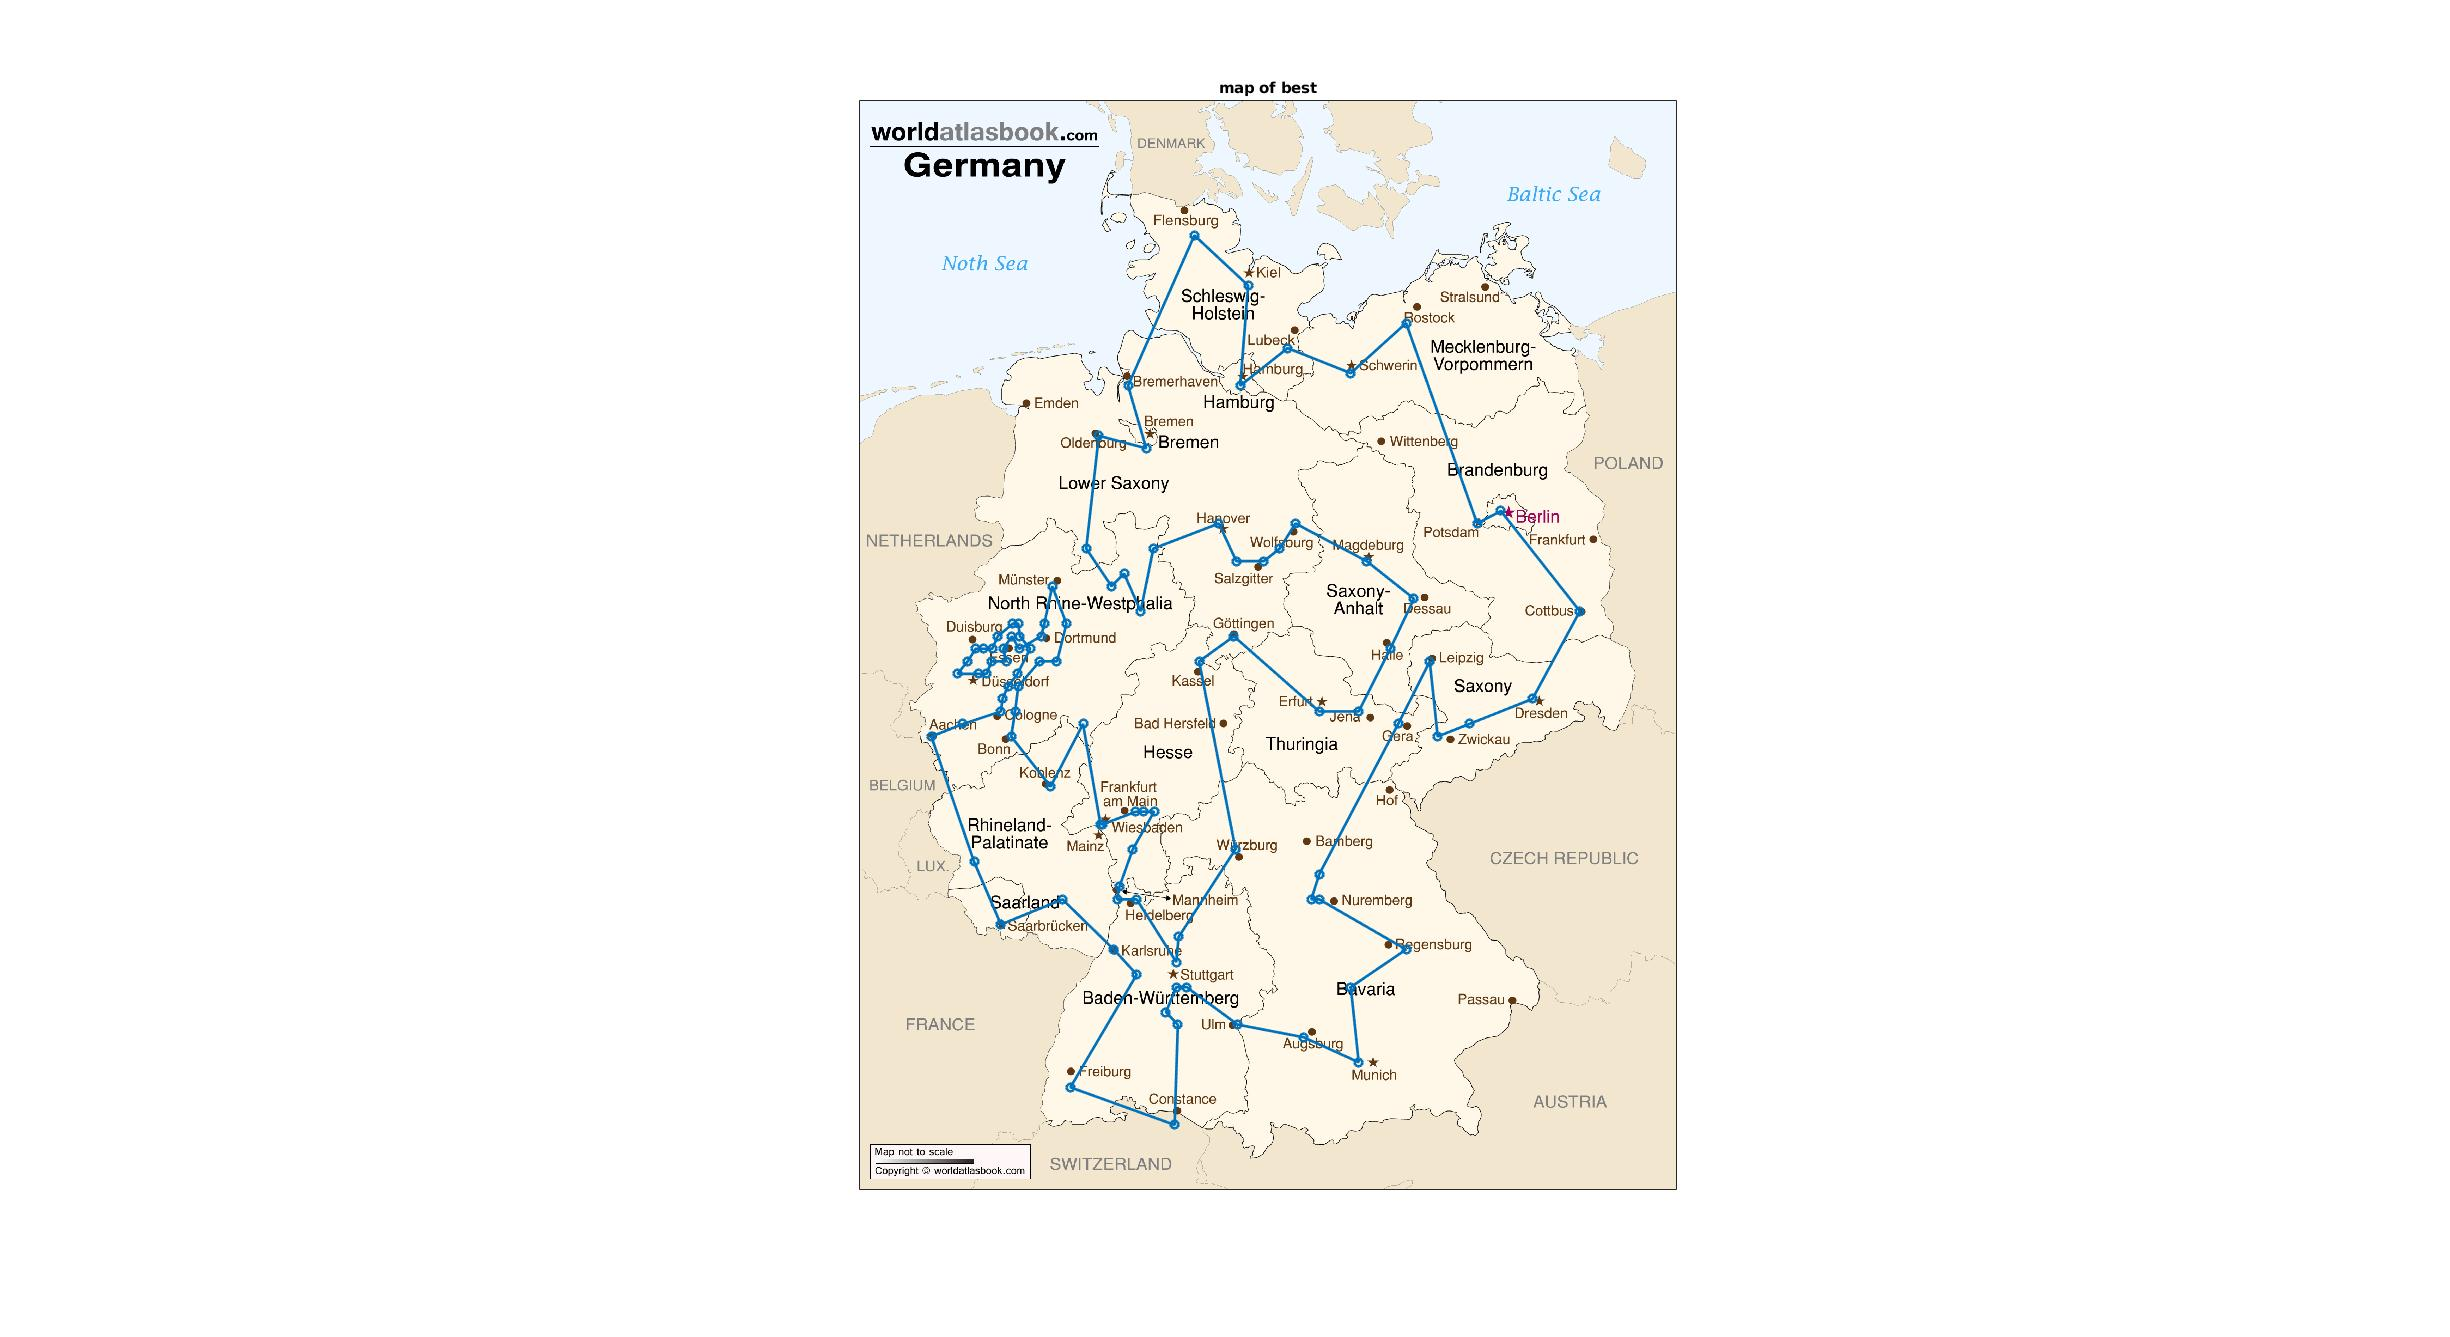
\includegraphics[width=1.0\textwidth]{images/BestPath_ultimate.jpg}
    \caption{Absolute best map \label{fig:xxx1}}
\end{figure}

\newpage
\subsection{Different crossover rates}

\begin{figure}[ht!]
	\centering
	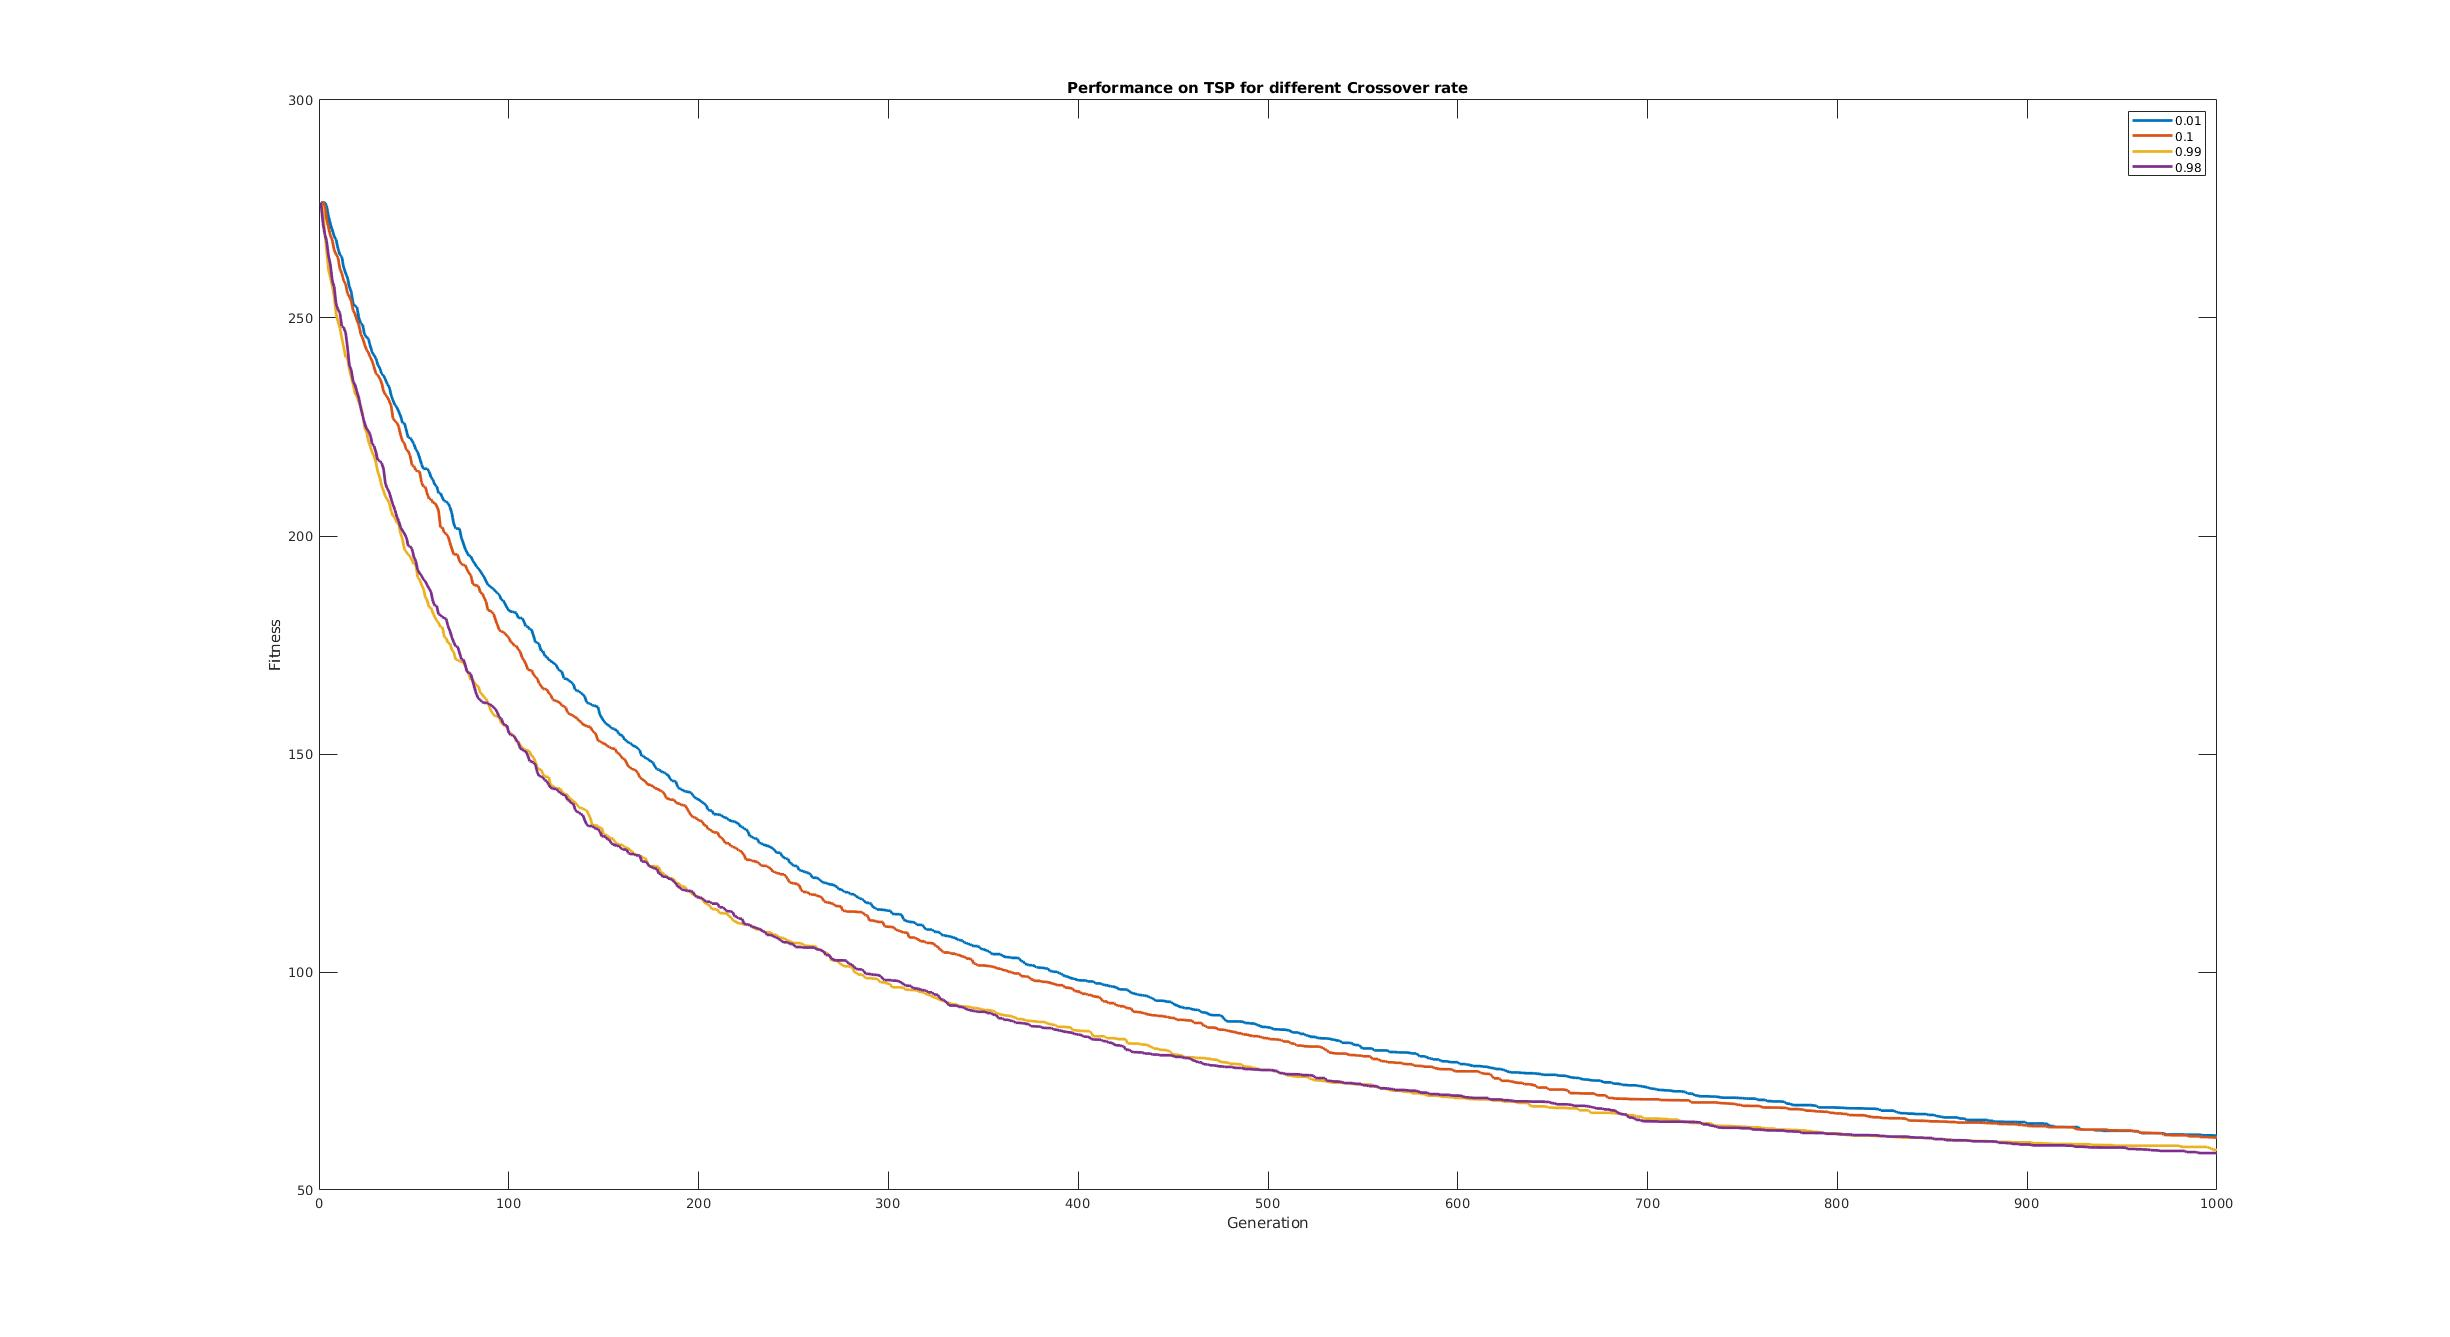
\includegraphics[width=1.0\textwidth]{images/crossover_exp_98.jpg}
	\caption{Crossover rate comparision\label{fig:crossfig}}
\end{figure}

Describe and explain the different mutation rates and how they influence the learning behaviour. Please remember to also focus on why, not only on what.
Also elaborate on the mutation rate you have chosen as best mutation rate.
\begin{itemize}
    \item We perform single point crossover.
    \item We choose \texttt{sp} individuals and select one with best fitness as father. We choose the mother in the same way.
    \item We select a \texttt{crossPoint} at random and select \texttt{1:crossPoint} genes from father's genotype and remaining genes are added in the order in which they appear in mother's genotype.
    \item We have discovered that crossover rate of 98\% performs best.
    \item As the crossover rate increases, the means fitness becomes better and better. This is expected, because when the rate is high, the child will have higher chance of getting better genes from 2 parents but when the rate is low, child will probably be just a copy of father.
    \item As it is seen in Figure~\ref{fig:crossfig}, 98\% crossover rate experiment performs almost same with 99\% but slightly better at the very end.
\end{itemize}

\newpage

\subsection{Different mutation rates}


\begin{figure}[ht!]
  \centering
  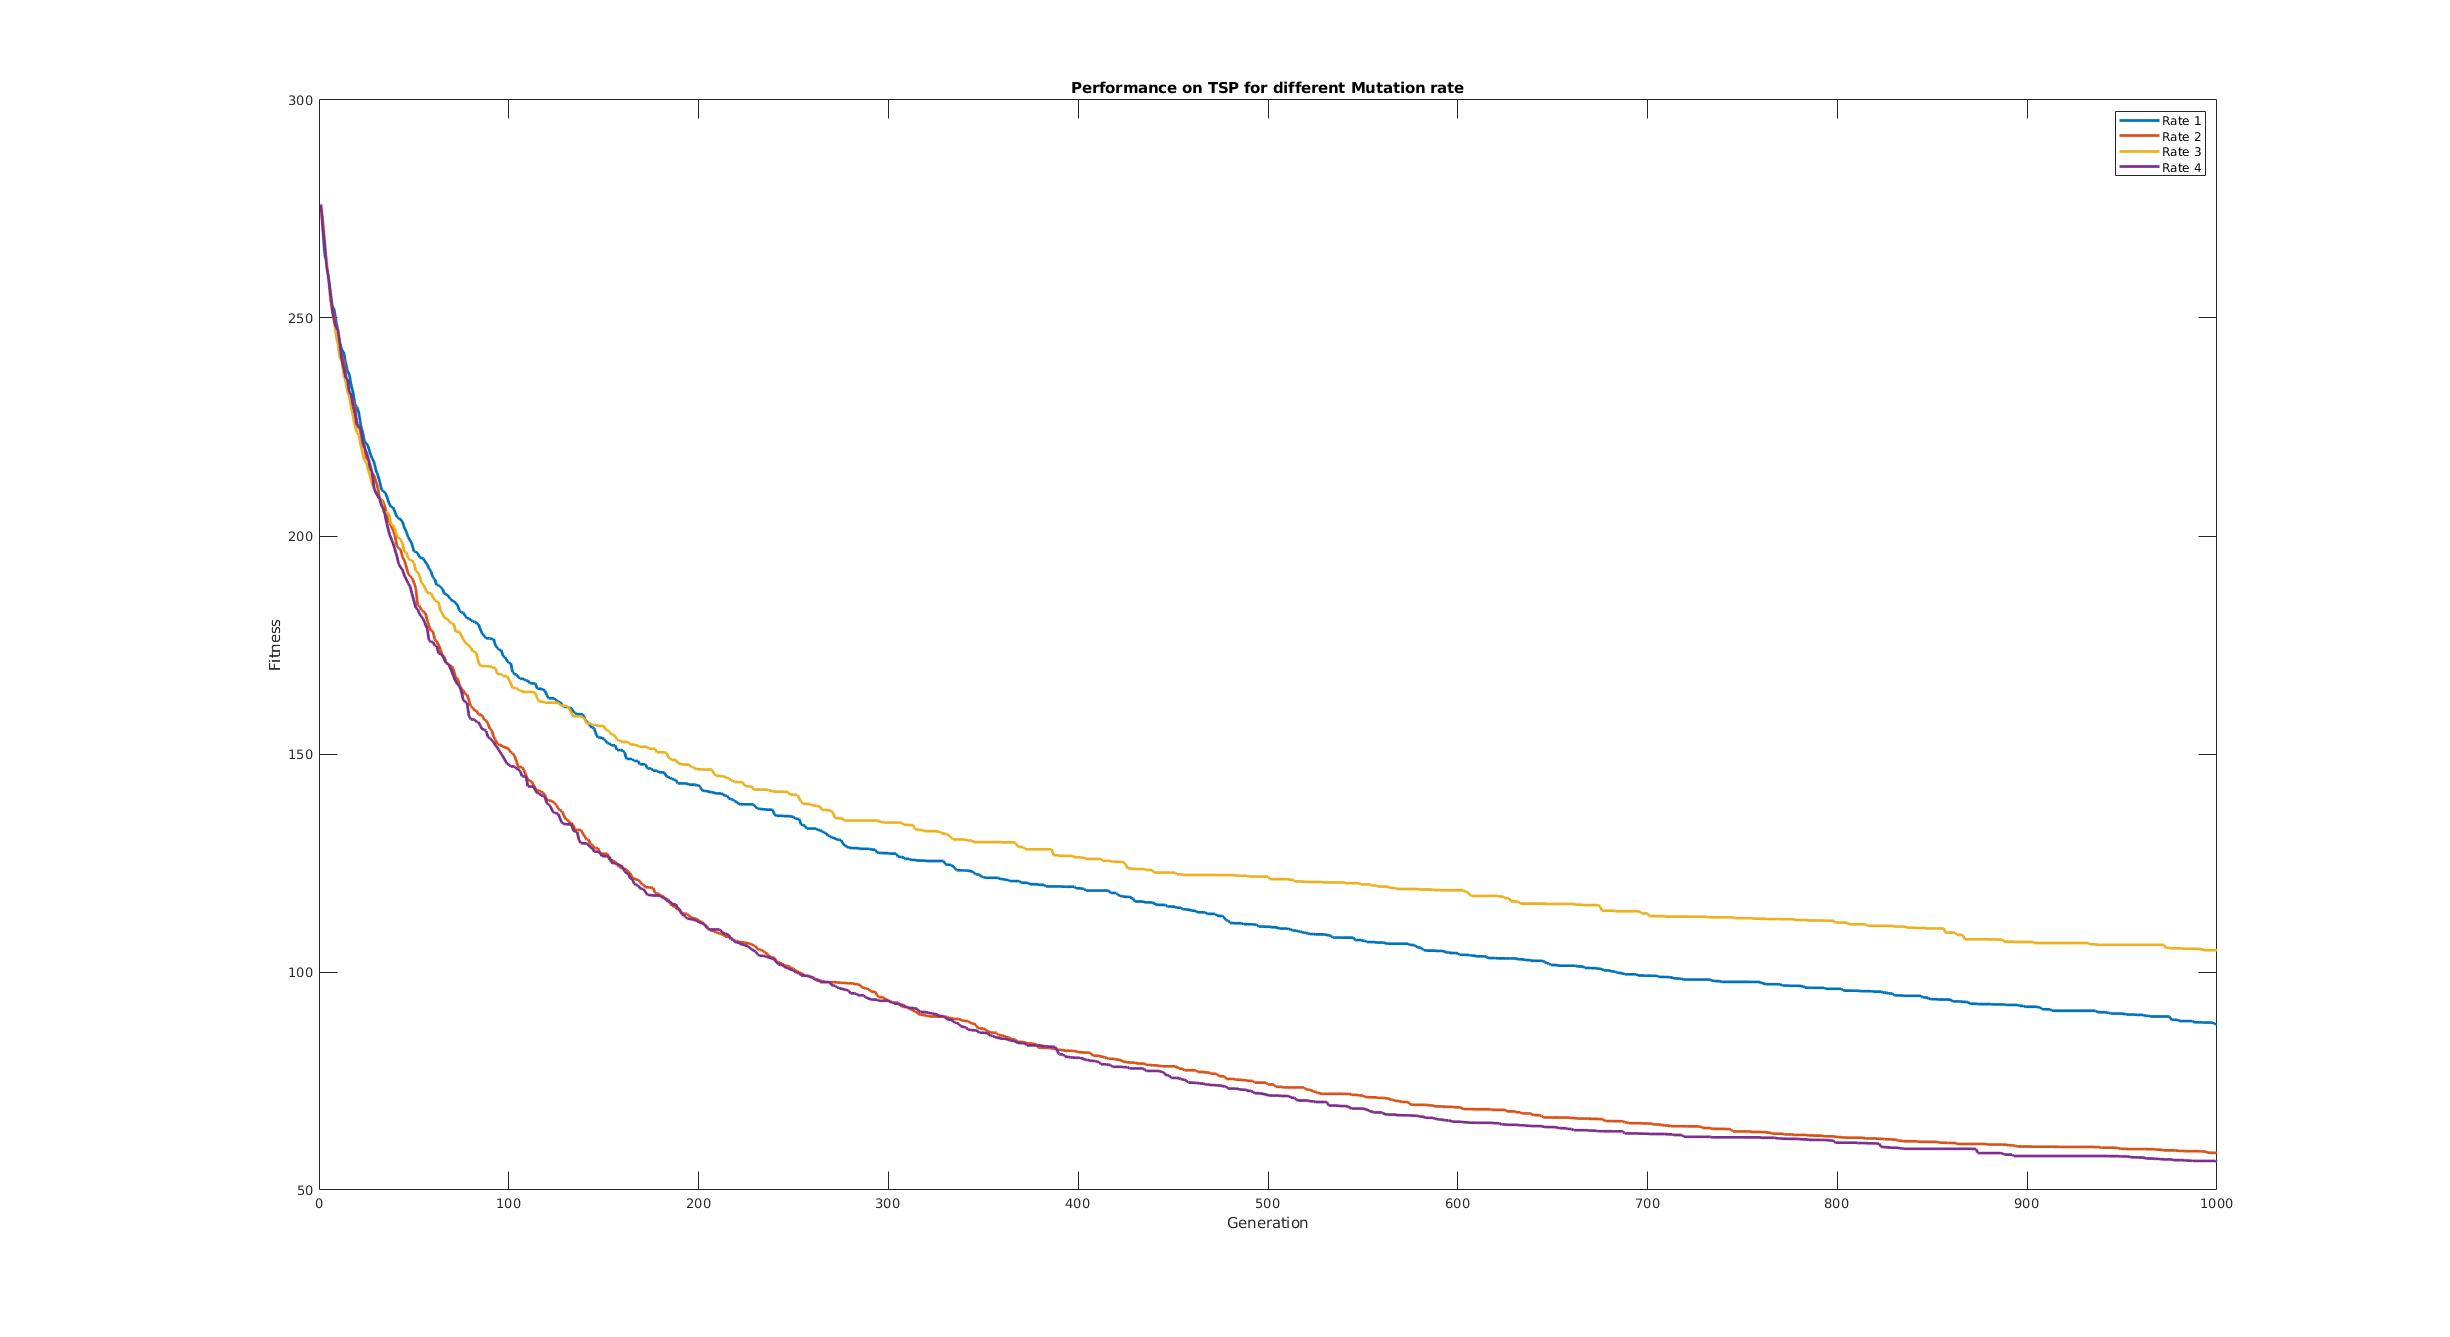
\includegraphics[width=1.0\textwidth]{images/mutation_exp_25.jpg}
    \caption{Mutation rate comparision\label{fig:mutfig}}
\end{figure}

Describe and explain the different crossover rates and how they influence the learning behaviour. Please remember to also focus on why, not only on what.
Also elaborate on the crossover rate you have chosen as best mutation rate.
\begin{itemize}
    \item We perform \textit{partial shuffle mutation}.
    \item We mutate an individual with \texttt{mutProb} probability.
    \item We select two points \textit{i,j}. We reverse the gene string between \textit{i} and \textit{j}.
    \item We have discovered that mutation rate of 25\% performs best.
    \item The reason for this is because 25\% is optimal. If the rate is higher than it disrupts the progress of generation and if it is lower than it is not enough progress.
\end{itemize}

\begin{figure}[ht!]
  \centering
  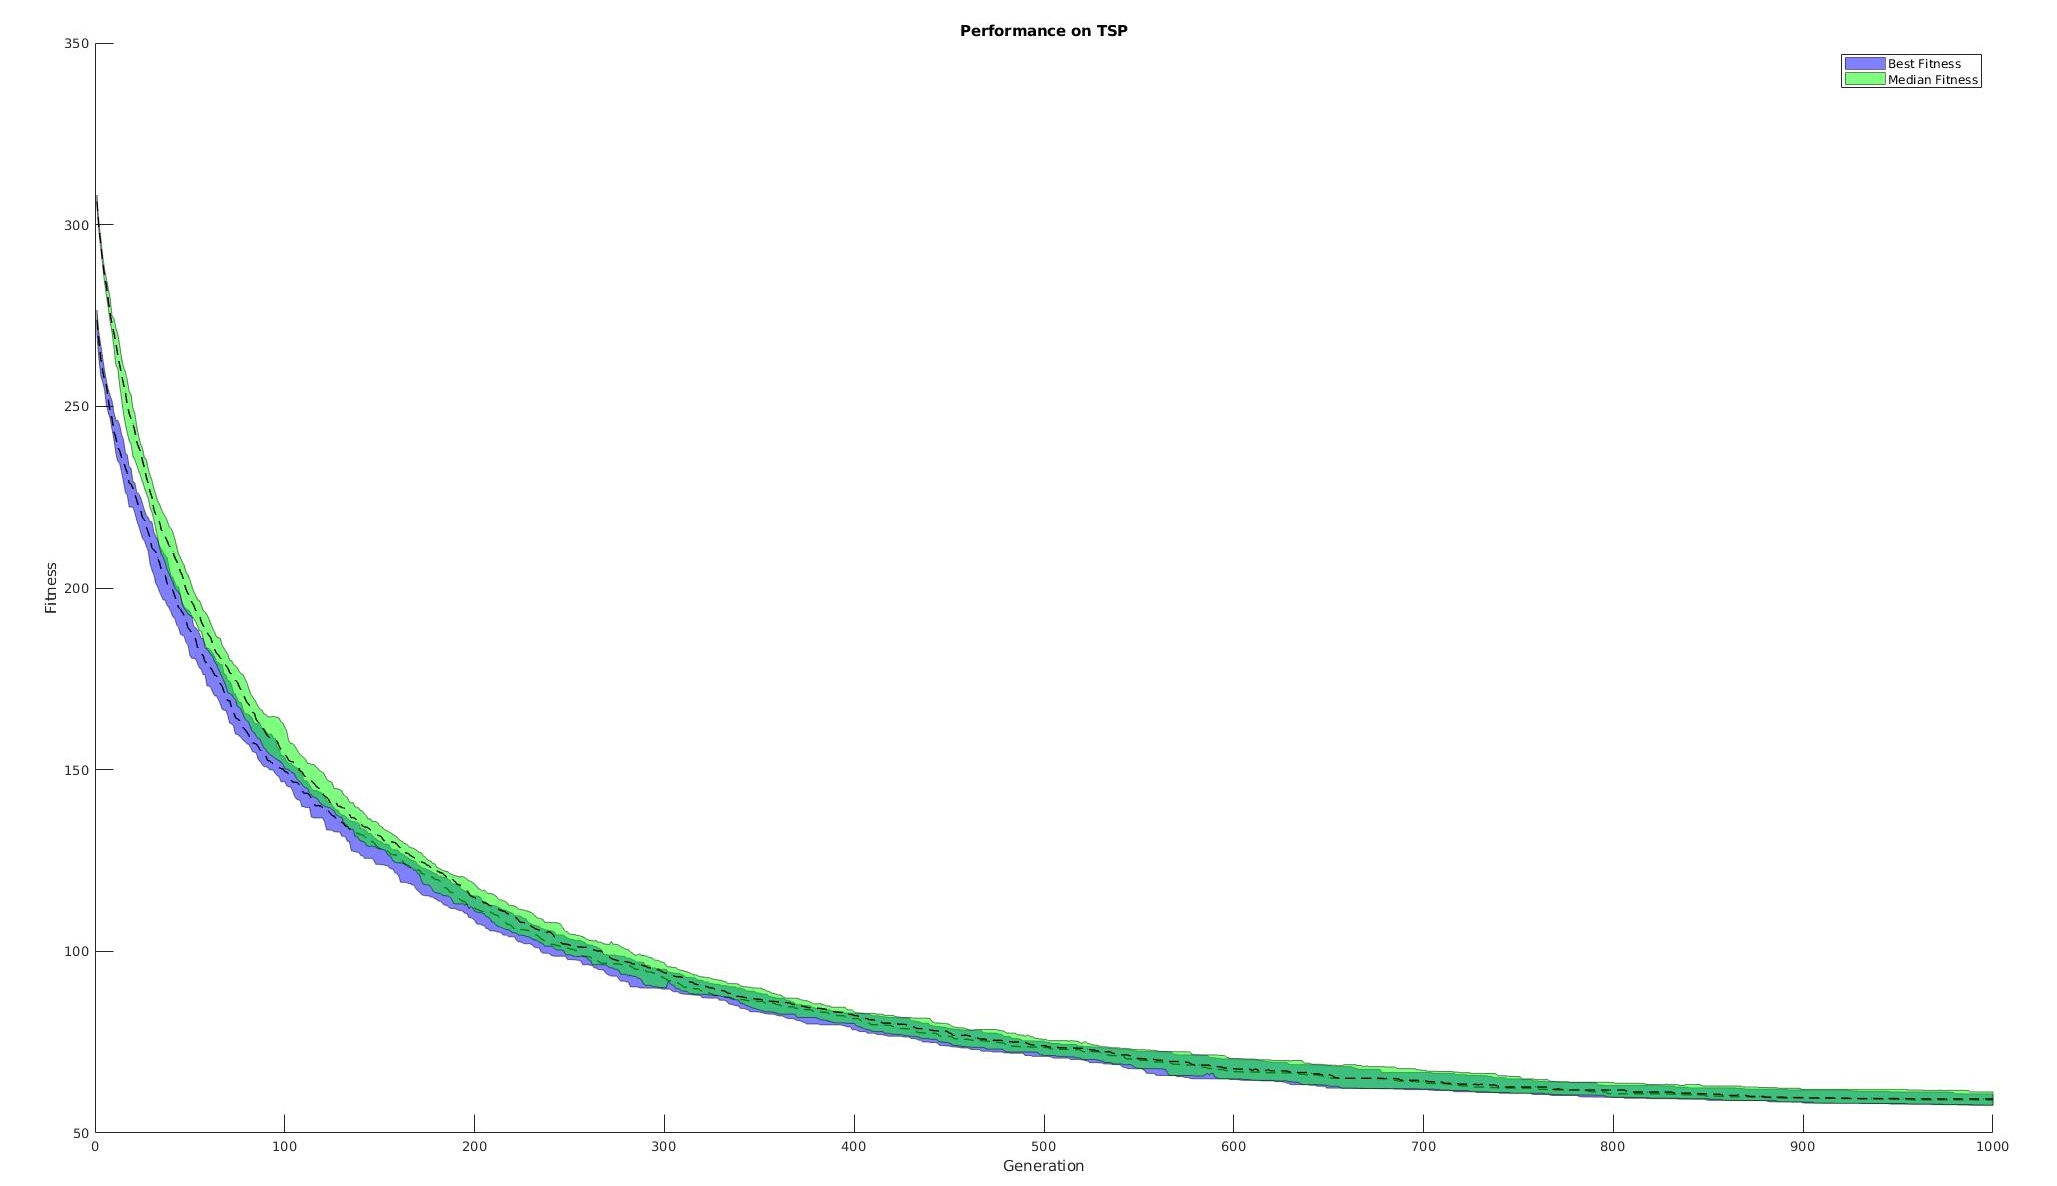
\includegraphics[width=1.0\textwidth]{images/1000X30_updated.jpg}
  \caption{Best and median fitness over 30 Experiments\label{fig:mutfig}}
\end{figure}


\end{document}
